\begin{figure}
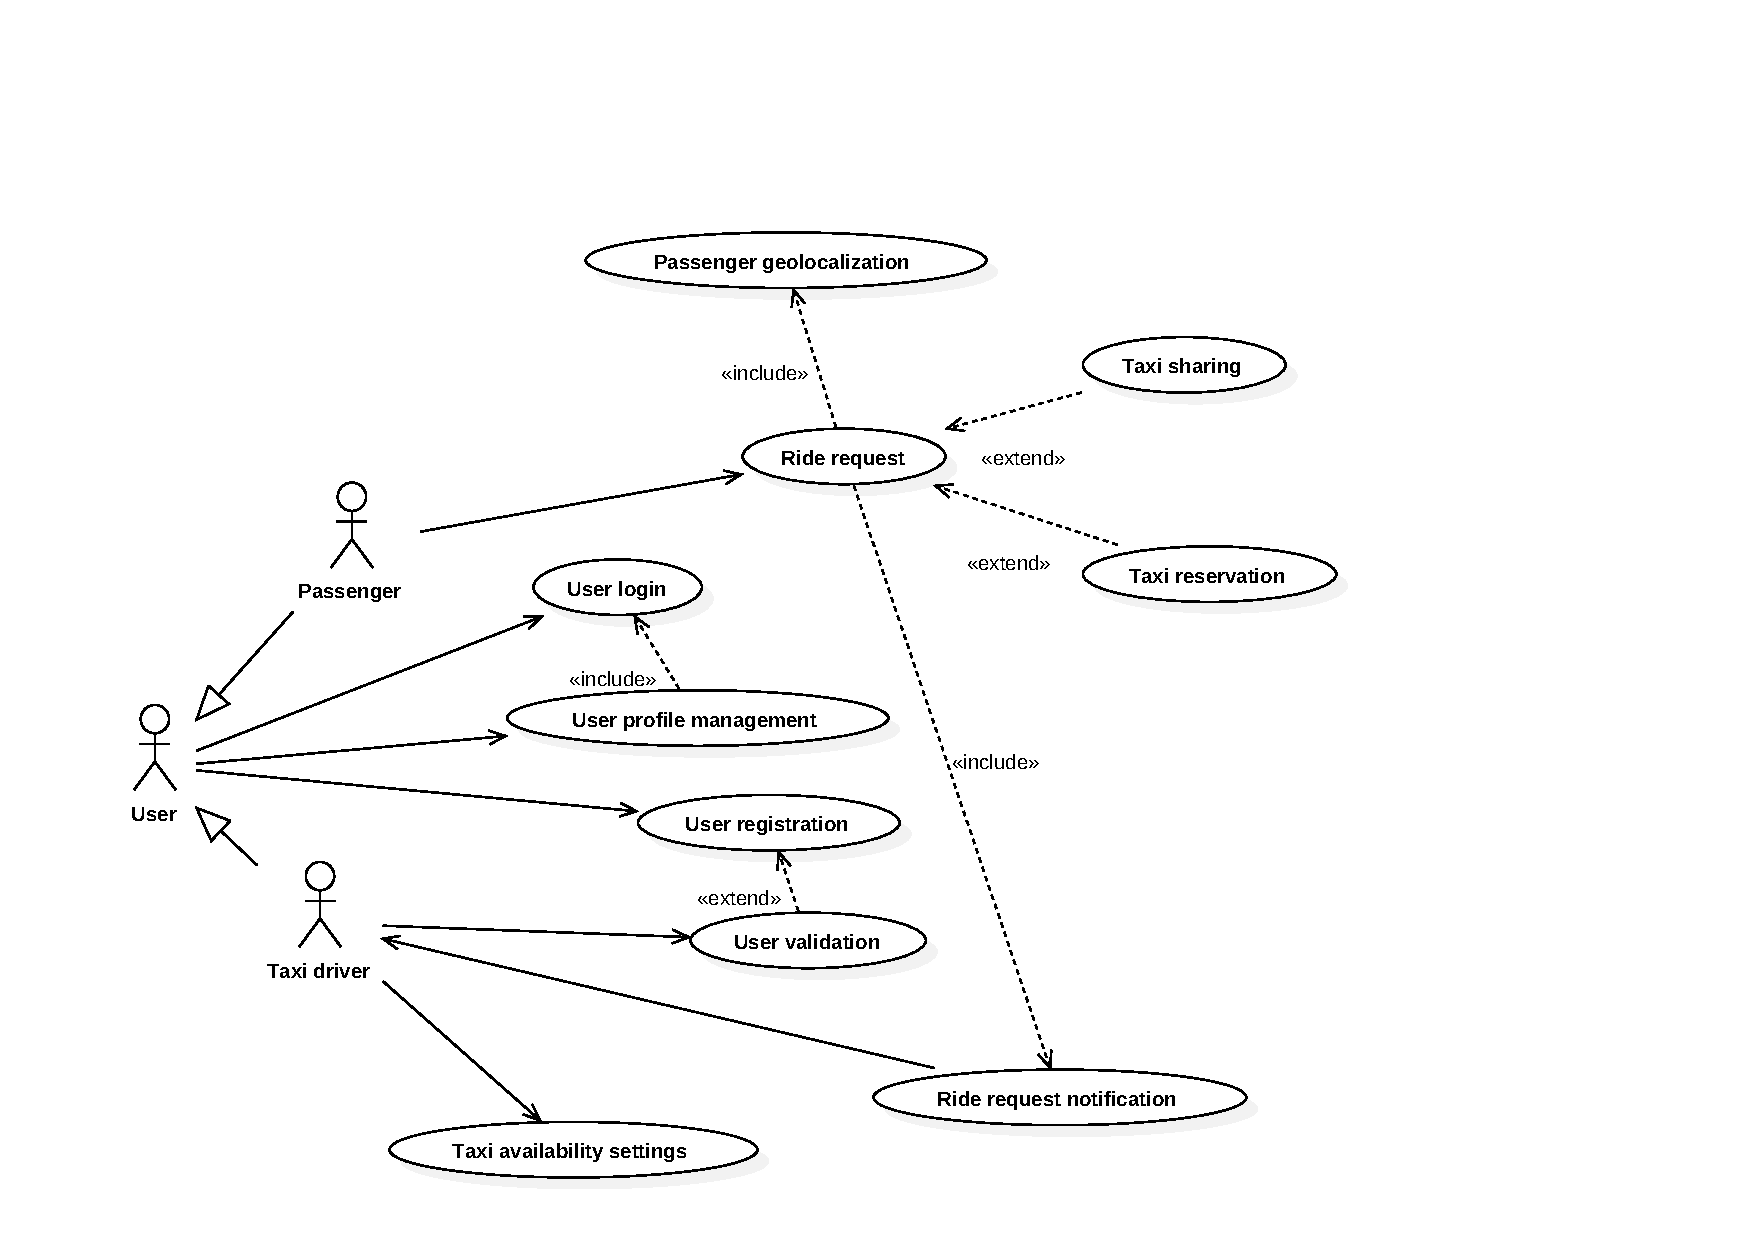
\includegraphics[width=\textwidth]{diagrams/usecase_whole.pdf}
\caption{The comprehensive use-case diagram of all the functionalities implemented by the system.}
\end{figure}

\begin{figure}
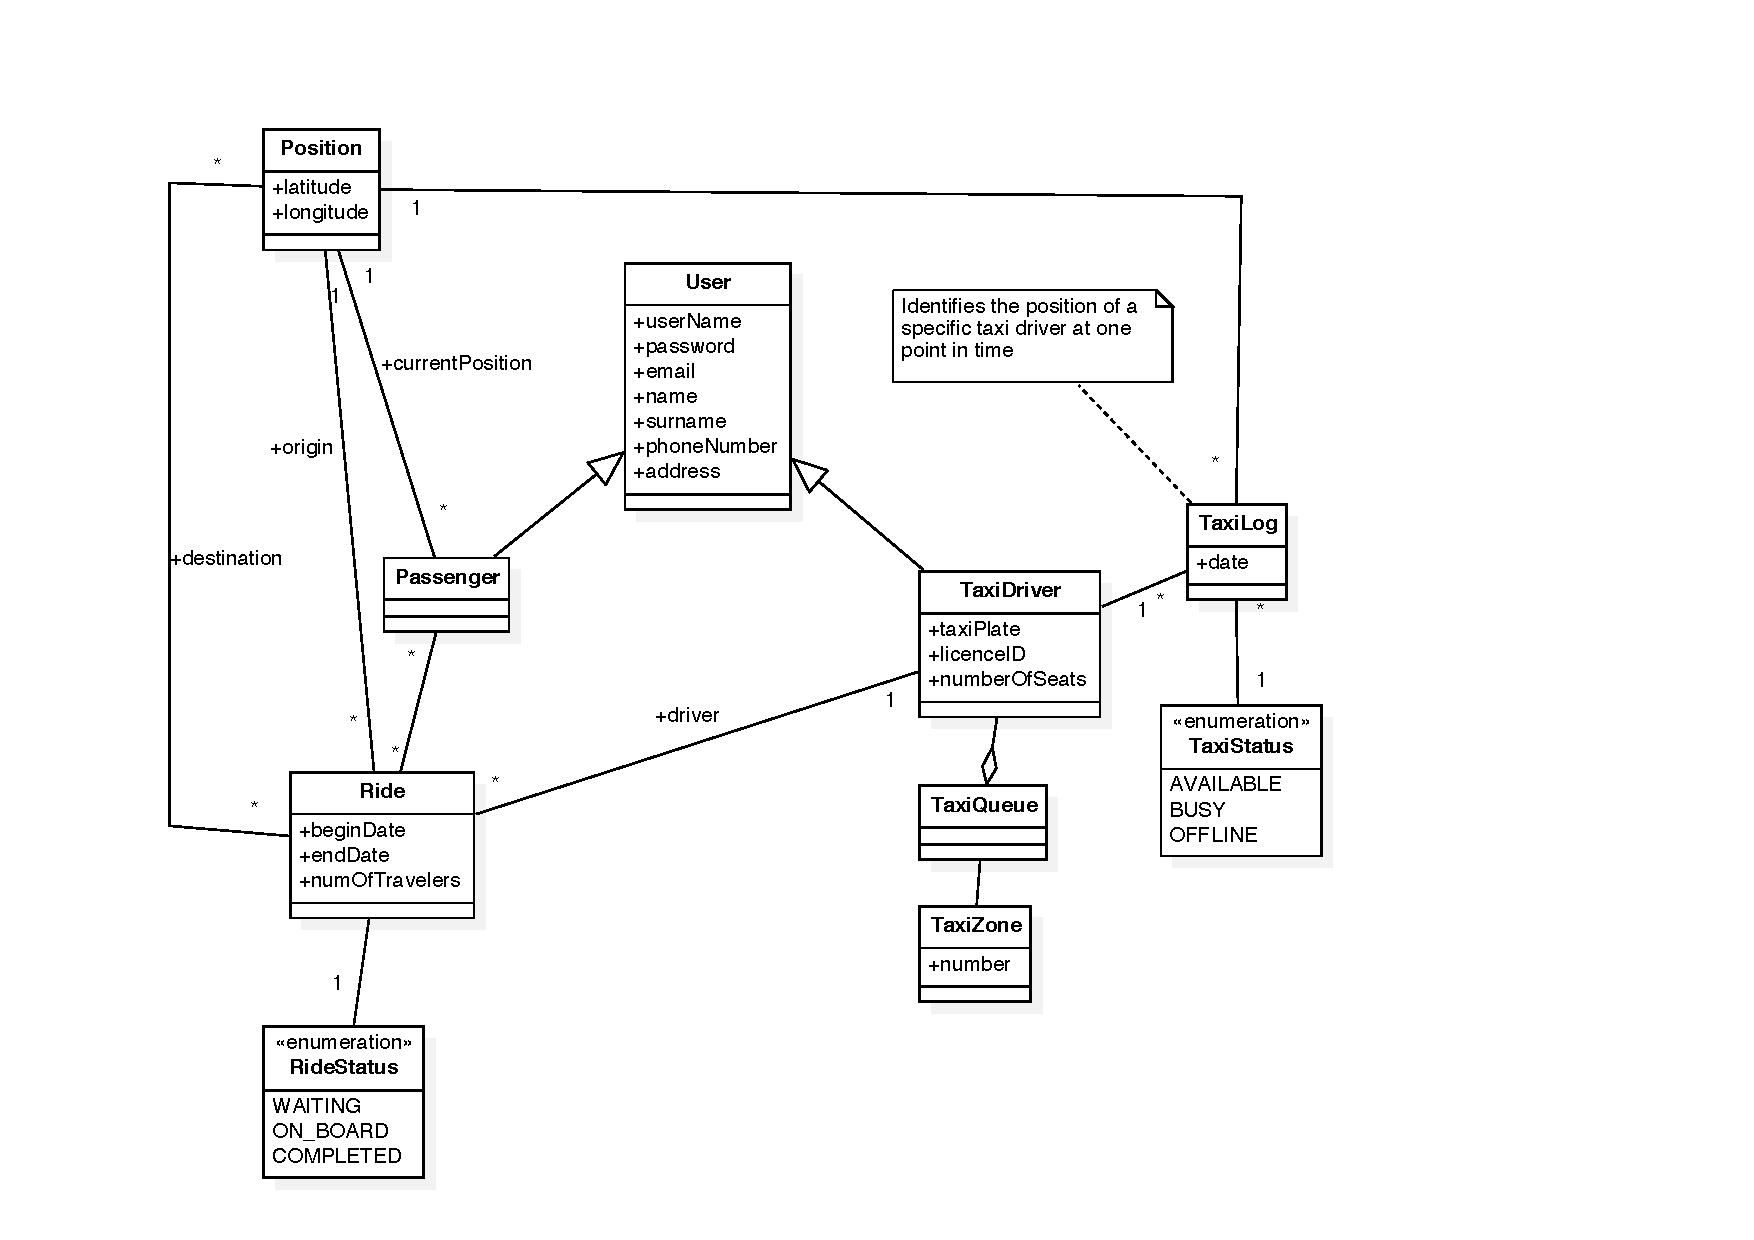
\includegraphics[width=\textwidth]{diagrams/general_class_diagram.pdf}
\caption{The comprehensive class diagram of the system.}
\end{figure}
The system allows passengers to book a taxi, and taxi drivers to take care of the request.

This is a list of what the users of the service can do.
\begin{itemize}
    \item All users can:
        \begin{itemize}
            \item create an account
            \item login
            \item edit profile data
            \item delete their account
        \end{itemize}
    \item Passengers can:
        \begin{itemize}
            \item request a taxi
            \item share a taxi with other passengers
            \item reserve a taxi in advance for a specific time
        \end{itemize}
    \item Taxi drivers can:
        \begin{itemize}
            \item mark themselves as available or busy
            \item accept or deny a lift request
            \item get the exact position of the passenger, after having accepted a ride request
        \end{itemize}
\end{itemize}
